\documentclass[runningheads]{llncs}

\usepackage{graphicx}
\usepackage{times}
\usepackage{rotate}
\usepackage{lscape}

%% MES PACKAGES/COMMANDES

\usepackage{amsmath}
\usepackage{amsfonts}
\usepackage{amssymb}
\usepackage{multicol}
\usepackage{mathenv}
\usepackage[utf8]{inputenc}

\usepackage[french]{babel}
\selectlanguage{french}

\usepackage{color}
%\usepackage{hyperref}
%\hypersetup{pdfborder={0 0 0}, colorlinks=true, urlcolor=blue, linkcolor = darkred}
\usepackage{verbatim}
\usepackage{moreverb}

\definecolor{darkred}{rgb}{0.85,0,0}
\definecolor{darkblue}{rgb}{0,0,0.7}
\definecolor{darkgreen}{rgb}{0,0.6,0}
\definecolor{darko}{rgb}{0.93,0.43,0}
\definecolor{maintitle}{rgb}{0.66,0,0.22}
\definecolor{title}{rgb}{0,0.5,0.5}

\newcommand{\maintitlecolor}[1]{\textcolor{maintitle}{#1}}
\newcommand{\titre}[1]{\textcolor{title}{#1}}
\newcommand{\tsect}[1]{\titre{\section{#1}}}
\newcommand{\tssect}[1]{\titre{\subsection{#1}}}
\newcommand{\tsssect}[1]{\titre{\subsubsection{#1}}}
\newcommand{\vect}[1]{\overrightarrow{#1}}
\newcommand{\dred}[1]{\textcolor{darkred}{\textbf{#1}}}
\newcommand{\dgre}[1]{\textcolor{darkgreen}{\textbf{#1}}}
\newcommand{\dblu}[1]{\textcolor{darkblue}{\textbf{#1}}}
\newcommand{\dora}[1]{\textcolor{darko}{\textbf{#1}}}
\newcommand{\gre}[1]{\textcolor{darkgreen}{#1}}
\newcommand{\blu}[1]{\textcolor{darkblue}{#1}}
\newcommand{\ora}[1]{\textcolor{darko}{#1}}
\newcommand{\rouge}[1]{\textcolor{darkred}{#1}}
\newcommand{\ceil}[1]{\left\lceil #1 \right\rceil}
\newcommand{\cdil}[1]{\left\lfloor #1 \right\rfloor}
\newcommand{\term}[1]{\textit{\textcolor{maintitle}{#1}}}
\newcommand{\image}[1]{\includegraphics{#1}}
\newcommand{\imageR}[2]{\includegraphics[width=#2px]{#1}}
\newcommand{\imageRT}[2]{\includegraphics[height=#2px]{#1}}
\newcommand{\img}[1]{\begin{center}\includegraphics[width=400px]{#1}\end{center}}
\newcommand{\imag}[1]{\begin{center}\includegraphics{#1}\end{center}}
\newcommand{\imgR}[2]{\begin{center}\includegraphics[width=#2px]{#1}\end{center}}
\newcommand{\imgRT}[2]{\begin{center}\includegraphics[height=#2px]{#1}\end{center}}
\newcommand{\point}[2]{\item \ora{\underline{#1}} : \textit{#2}}
\newcommand{\bfp}[2]{\item \textbf{#1} : \textit{#2}}
\newcommand{\sumparam}[3]{\sideset{}{_{#1}^{#2}}\sum{#3}}
\newcommand{\sumin}[3]{\sideset{}{_{i=#1}^{#2}}\sum{#3}}
\newcommand{\sumkn}[3]{\sideset{}{_{k=#1}^{#2}}\sum{#3}}
\newcommand{\intin}[3]{\sideset{}{_{#1}^{#2}}\int{#3}}
\newcommand{\stitre}[1]{\noindent\textbf{\underline{#1}} \\}
\newcommand{\R}{\mathbb{R}}
\newcommand{\Z}{\mathbb{Z}}
\newcommand{\N}{\mathbb{N}}
\newcommand{\ualpha}{\vect{u_\alpha}}
\newcommand{\valpha}{\vect{v_\alpha}}
\newcommand{\palpha}{\vect{\Psi_\alpha}}
\newcommand{\npcomp}{\term{$\mathcal{NP}$-complet}}
\newcommand{\npcompl}{\term{$\mathcal{NP}$-complet} }

%% FIN MES PACKAGES/COMMANDES

%% DEBUT DU DOCUMENT

\begin{document}

\frontmatter          % for the preliminaries
\pagestyle{headings}  % switches on printing of running heads
\mainmatter              % start of the contributions
\title{Gestion de Projet Informatique 2000-2010\\
Rapport de Planification}

\titlerunning{Gestion de projet informatique -- Rapport de planification}

\author{DUBUC XAVIER}
%
\authorrunning{DUBUC XAVIER - 1e ann\'ee du master en sciences informatiques} 

\institute{Premi\`ere ann\'ee du grade de master en sciences informatiques\\
Facult\'e des Sciences, Universit\'e de Mons\\
Av. du champ de Mars 6, 7000 Mons, Belgium\\
\email{XAVIER.DUBUC@student.umons.ac.be}
}
\frontmatter          % for the preliminaries
\pagestyle{headings}  % switches on printing of running heads
\mainmatter              % start of the contributions
\title{Gestion de Projet Informatique 2000-2010\\
Rapport de Planification}

\titlerunning{Gestion de projet informatique -- Rapport de planification}

\author{DUBUC XAVIER}
%
\authorrunning{DUBUC XAVIER - 1e ann\'ee du master en sciences informatiques} 

\institute{Premi\`ere ann\'ee du grade de master en sciences informatiques\\
Facult\'e des Sciences, Universit\'e de Mons\\
Av. du champ de Mars 6, 7000 Mons, Belgium\\
\email{XAVIER.DUBUC@student.umons.ac.be}
}

\maketitle              % typeset the title of the contribution

\begin{center} \today \end{center}
\begin{abstract}
Ce rapport est rendu dans le cadre du cours de ``Gestion de Projets Logiciels" (dispens\'e par Monsieur \emph{Tom Mens} en ann\'ee 
acad\'emique 2010-2011). Le but de ce rapport est d’énoncer les ressources matérielles et humaines nécessaires ainsi que 
les contraintes de temps, de budget et de fonctionnalité du projet.

\end{abstract}

%%%%%%%%%%%%%%%%%%%%%%%%%%%%%%%%%%%%%%%%%%%%%%%%
%%%%%%%%%%%%%%%%%%%%%%%%%%%%%%%%%%%%%%%%%%%%%%%%
\maketitle              % typeset the title of the contribution

\begin{center} \today \end{center}
\begin{abstract}
Ce rapport est rendu dans le cadre du cours de ``Gestion de Projets Logiciels" (dispens\'e par Monsieur \emph{Tom Mens} en ann\'ee 
acad\'emique 2010-2011). Le but de ce rapport est d’énoncer les ressources matérielles et humaines nécessaires ainsi que 
les contraintes de temps, de budget et de fonctionnalité du projet.

\end{abstract}

%%%%%%%%%%%%%%%%%%%%%%%%%%%%%%%%%%%%%%%%%%%%%%%%
%%%%%%%%%%%%%%%%%%%%%%%%%%%%%%%%%%%%%%%%%%%%%%%%
\section{Introduction}\label{sec:intro}

\subsection{Objectifs}

Le travail consiste à lire, comprendre et implémenter une méthode récente de recherche du nombre chromatique d'un graphe, la 
recherche dans des espaces variables, proposée par \textit{Hertz} et al [1]. Pour rappel, le nombre chromatique d'un graphe est le 
nombre de couleur minimum nécessaires à la coloration de ses sommets de telle manière que des sommets adjacents n'aient pas la 
même couleur.

%%%%%%%%%%%%%%%%%%%%%%%%%%%%%%%%%%%%%%%%%%%%%%%%
\subsection{Exigences fonctionnelles}

Le logiciel devra être capable de réussir les tests effectués sur des instances réputées difficiles (DIMACS challenges [2]) et, 
si le temps le permet, applicable sur protoype simple de logiciel de planification d'horaire d'examens.

%%%%%%%%%%%%%%%%%%%%%%%%%%%%%%%%%%%%%%%%%%%%%%%%
\subsection{Exigences non-fonctionnelles}

Aucune exigence quant à la portabilité mais le projet sera implementé à JAVA afin de nous assurer cette portabilité tout de même, 
il va sans dire que les structures de données et algorithmes implementés devront être optimisés afin de diminuer les temps de 
calcul.

%%%%%%%%%%%%%%%%%%%%%%%%%%%%%%%%%%%%%%%%%%%%%%%%
\subsection{Contraintes de temps}

\emph{Y a-t-il des contraintes sur l'emploi du temps? (Dates d'\'ech\'eance, vacances, examens, autres)? Si vous le d\'esirez vous pouvez utiliser une table ici pour clarifier l'emploi du temps. Vous pouvez \'egalement ajouter une figure.}

Il y a 3 échéances au total,
\begin{itemize}
\item le \textbf{28 octobre 2010}, date où il faut rendre le rapport de planification qui devra donc être fini avant cette date. 
Ceci implique que la compréhension du projet, les démarches administratives, ainsi que la planification doivent être terminés 
avant cette date.
\item début \textbf{janvier 2011}, date où il faudra rendre le prérapport, ceci implique donc que toutes les recherches et autres 
préliminaires ou prémisces (conception, ...) doivent être finis avant cette date afin que ces résultats soient incorporés au 
rapport.
\item \textbf{mai 2011}, date que nous nous fixons pour rendre le dernier livrable, c'est-à-dire le programme implémenté, testé et 
débuggé, devant rendre le rapport pour le mois de juin, il convient de nous laisser une plage de temps acceptable pour la 
rédaction de celui-ci.
\end{itemize}

%%%%%%%%%%%%%%%%%%%%%%%%%%%%%%%%%%%%%%%%%%%%%%%%
\subsection{Contraintes de budget}

Le logiciel n'utilisant que JAVA comme base et les DIMACS challenge n'étant également pas payant, aucune contrainte budgétaire 
n'est à remarquer.

%%%%%%%%%%%%%%%%%%%%%%%%%%%%%%%%%%%%%%%%%%%%%%%%
%%%%%%%%%%%%%%%%%%%%%%%%%%%%%%%%%%%%%%%%%%%%%%%%
\section{Ressources}\label{sec:organisation}

\subsection{Les ressources humaines (personnel)}

\begin{itemize}
\item \term{Le responsable des projets} \textit{(Tom Mens)} s'occupe de la validation des choix de projets et de l'établissement 
du calendrier. C'est également lui qui résoud les éventuels problèmes liés à l'organisation.
\item \term{Le directeur de projet} \textit{(Hadrien Melot)} oriente l'étudiant vers la documentation nécéssaire à 
l'accomplissement du projet, il s'assure également que ce projet est réalisable dans les délais. Il fait également partie de ceux
qui évaluent le travail final après sa remise. \textit{(Il établit également, avec l'étudiant, le cahier des charges)}
\item \term{L'étudiant} \textit{(Xavier Dubuc)} réalise le travail, il se documente, lit et comprend cette documentation ; écrit 
des rapports à intervals fixés, développe l'application en choisissant des outils (ou en utilisant ceux imposés) pour mener le 
projet à bien. C'est lui le responsable du travail et du rapport final.
\item \term{Le(s) rapporteur(s)} \textit{(Véronique Bruyère et ?)} complètent l'équipe qui évaluera le travail de l'étudiant après 
sa remise, cette évaluation sera donc basée sur le travail en lui même, le rapport final ainsi que sa présentation.
\end{itemize}

%%%%%%%%%%%%%%%%%%%%%%%%%%%%%%%%%%%%%%%%%%%%%%%%
\subsection{Les ressources logicielles}

L'application sera développée en \textbf{JAVA}, cette application ne nécessite aucune librairie supplémentaire ni de programmes 
complémentaires. \textbf{JAVA} étant \textit{OpenSource}, aucun coût n'est donc à imputer, comme spécifié dans la section des 
contraintes de budget.

%%%%%%%%%%%%%%%%%%%%%%%%%%%%%%%%%%%%%%%%%%%%%%%%
\subsection{Les ressources mat\'erielles}

La machine de développement sera celle de l'étudiant \textit{(\textbf{ASUS X64J}, Intel Core i3-350M (2,26 GHz), 4Gb DDR 3)}
doté d'un dual boot Windows 7even/Ubuntu 10.04 (probablement 10.10 prochainement) permettant de tester la compatibilité de 
l'application sous Windows et Linux (pour tester la portabilité).

%%%%%%%%%%%%%%%%%%%%%%%%%%%%%%%%%%%%%%%%%%%%%%%%
%%%%%%%%%%%%%%%%%%%%%%%%%%%%%%%%%%%%%%%%%%%%%%%%
\newpage
\section{Analyse des risques}

\subsection{Identification des risques}\label{sec:riskident}

\begin{table}[!htbp]
\begin{center}
\begin{tabular}{|p{3cm}||c|c|}
\hline
\textbf{Risque} & Probabilit\'e & S\'ev\'erit\'e\\
\hline\hline
Difficultés d'implémentation des structures & basse &  \large{s\'erieuse} \\
\hline
Mauvaise compréhension d'un concept & basse &  \large{s\'erieuse} \\
\hline
Problème de gestion du temps & \large{mod\'er\'ee} & tol\'erable \\
\hline
Produit final défectueux & \large{mod\'er\'ee} & \Large{sérieuse} \\
\hline
\end{tabular}
\end{center}
   \caption{Analyse des risques.}
   \label{tab:risques}
\end{table}

L'implémentation des structures et la compréhension des concepts étant la base même du projet, une quelconque erreur dans ces 2
domaines peuvent entraîner une perte de qualité certaines ainsi qu'un retard considérable (par exemple si une structure est mal 
implémentée, le produit final sera plus lent et si un concept est mal compris, l'algorithme ne fonctionnera pas et il faudra le 
débugger). Heureusement ces risques sont de probabilité faible car l'implémentation des structures (graphes) a déjà été fait les 
années précédentes et ne devrait pas poser de problème. La compréhension des concepts, au vu des concepts utilisés qui sont 
relativement simples ne devraient pas poser de problème non plus. \\

La gestion du temps sera pour le moins délicate, car nous aurons à gérer tous les autres travaux qui nous seront demander en plus 
de celui-ci et un retard est vite arrivé dans ces cas-là ; ce risque reste tolérable car on peut toujours rattraper un retard 
(tant qu'il n'est pas trop conséquent). \\

Le produit final défectueux quant à lui posera pas mal de souci également, vu qu'il y a beaucoup de concept à implémenter, le 
débugage ne sera pas aisé, que ce soit parce qu'il ne fonctionne pas ou parce qu'il est trop lent.

%%%%%%%%%%%%%%%%%%%%%%%%%%%%%%%%%%%%%%%%%%%%%%%%
\subsection{Gestion des risques}\label{sec:riskmanagement}

\begin{enumerate}
\item \term{Risque de difficultés d'implémentation des structures}, il convient, en vue de minimiser ce risque, de bien se 
documenter sur les structures employées ainsi que des meilleures manières de les implémenter. Ne pas hésiter à poser des questions 
si un choix n'est pas facile à prendre. Si malgré tout le risque est là, il faudra revoir toute l'implémentation de ces structures
afin de résoudre le problème occasionné.
\item \term{Risque de mauvaise compréhension d'un concept}, il convient de bien lire la documentation et de résumer chaque concept 
de manière à être capable de l'expliquer et de l'appliquer. Si malgré tout le risque est là, il conviendra de relire la 
documentation attentivement, en chercher de la nouvelle et/ou en parler avec le directeur de projet ou quelqu'un spécialisé dans 
ce domaine.
\item \term{Problème de gestion du temps}, il convient d'effectuer également une planification des autres projets et travaux à 
effectuer pour les autres cours afin de concorder avec celui-ci, il convient également de faire passer ce projet-ci avant les 
autres en cas de conflit. Si malgré tout le risque est là, il faudra travailler plus vite ou plus souvent pour rattraper le retard 
encourru.
\item \term{Produit final défectueux}, il convient de tester le programme assez souvent afin de ne pas avoir un énorme debug à 
faire au terme du projet. Si malgré tout le risque est là, une période de temps "ultimes corrections" est prévues en cas de 
besoin, celle-ci empêtrant un peu sur la rédaction du rapport final (voir diagramme de GANTT).
\end{enumerate}

%%%%%%%%%%%%%%%%%%%%%%%%%%%%%%%%%%%%%%%%%%%%%%%%
%%%%%%%%%%%%%%%%%%%%%%%%%%%%%%%%%%%%%%%%%%%%%%%%
\newpage
\section{R\'epartition du travail}

\subsection{Work Breakdown Structure}

\begin{table}[htbp]
\begin{center}
\begin{tabular}{|r|l||l|c|p{3cm}|}
\hline
\textbf{ID} & T\^ache & Dates & Responsable & Autre remarques\\
\hline\hline
T1 & Établir le cahier de charges & 18 octobre & L\'etudiant et le directeur & peut être sujet à modification \\
\hline
T2 & Rédiger le rapport de planification & 22 octobre & L'étudiant & doit être rendu pour le 28 octobre \\
\hline
T3 & Faire le conception de l'application & Novembre - & L'étudiant & \\ 
& & Début Décembre & & \\
\hline
T4 & Rédaction du pré-rapport & Décembre & L'étudiant & \\
\hline
T5 & Relecture du pr\'e-rapport & Début janvier &  Le directeur & \\
\hline
T6 & Implémentation et Tests & Janvier-Mai & L'étudiant & \\
\hline
T7 & Validation du projet & Début Mai & Le directeur & \\
\hline
T8 & Rédaction du rapport final & Mai & L'étudiant & \\
\hline
T9 & Relecture du rapport final & Fin Mai - Début Juin & Le directeur & \\
\hline
T10 & D\'epot du projet & Juin & L'étudiant & \\
\hline
T11 & D\'efense orale du projet & Juin & L'étudiant (et le directeur) & \\
\hline
\end{tabular}
\end{center}
   \caption{Tableau des t\^aches.}
   \label{tab:WBS}
\end{table}

%%%%%%%%%%%%%%%%%%%%%%%%%%%%%%%%%%%%%%%%%%%%%%%%
\subsection{Etapes cl\'es }

\begin{table}[htbp]
\begin{center}
\begin{tabular}{|c||c|c|}
\hline
Date & \'etape cl\'e & Livrables\\
\hline\hline
30 septembre 2010 & Entretien d'acceptation du projet & Engagement\\
\hline
28 octobre 2010 & R\'eunion d'inspection de la planification de projet & Rapport de planification  \\
\hline
Janvier 2011 & Réunion d'inspection de l'état d'avancement du projet & Pré-rapport \\
\hline
Mars 2011 & Réunion d'inspection de l'implémentation des structures & Code JAVA \\
\hline
Avril 2011 & Réunion d'inspection de l'implémentation des algorithmes & Code JAVA \\
\hline
Mai 2011 & Réunion d'inspection du produit final & Code JAVA \\
\hline
Juin 2011 & Remise du logiciel (après corrections éventuelles) & Code JAVA final \\
\hline
\end{tabular}
\end{center}
   \caption{Tableau d'\'etapes cl\'es.}
   \label{tab:TEC}
\end{table}

%%%%%%%%%%%%%%%%%%%%%%%%%%%%%%%%%%%%%%%%%%%%%%%%
%%%%%%%%%%%%%%%%%%%%%%%%%%%%%%%%%%%%%%%%%%%%%%%%
\newpage
\section{Ordonnancement}

\subsection{Diagramme GANTT}

\begin{figure}[!htb]
\begin{center}
  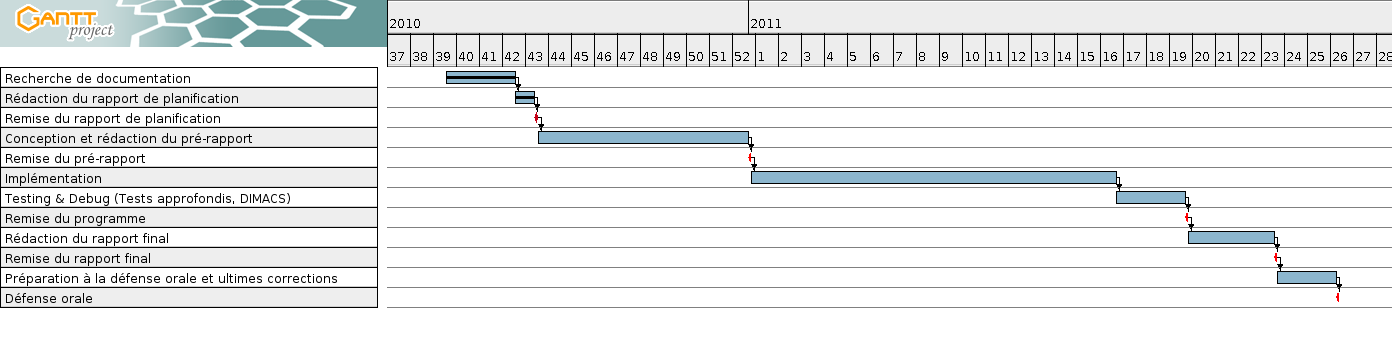
\includegraphics[width=\textwidth]{GANTT.png}
  \caption{Diagramme GANTT.}\label{fig:GANTT}
\end{center}
\end{figure}

%%%%%%%%%%%%%%%%%%%%%%%%%%%%%%%%%%%%%%%%%%%%%%%%
\subsection{Diagramme PERT}

\begin{figure}[!htb]
\begin{center}
  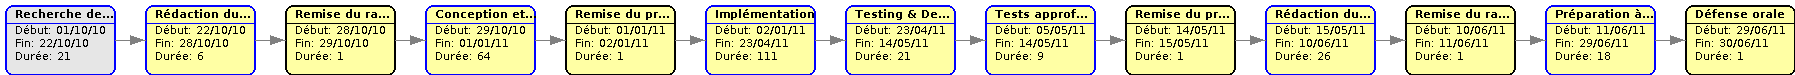
\includegraphics[width=\textwidth]{PERT.png}
  \caption{Diagramme PERT.}\label{fig:PERT}
\end{center}
\end{figure}

\begin{center}\textit{(voir TABLE 4)}\end{center}

\begin{table}[htbp]
\begin{center}
\begin{tabular}{|p{2cm}||c|c|c|c|c|c|}
\hline
\textbf{T\^ache} & Dur\'ee & Effort & Earliest Start & Latest Start & Slack Time & Free Float\\
\hline\hline
Recherche de documentation & 21 & 0,7 & 01/10/10 & 01/10/10 & 0 & 0 \\
\hline
Rédaction du rapport de planification & 6 & 0,2 & 22/10/10 & 22/10/10 & 0 & 0 \\
\hline
Remise du rapport de planification & 1 & 0,03 & 28/10/10 & 28/10/10 & 0 & 0 \\
\hline
Conception et rédaction du pré-rapport  & 64 & 2,13 & 29/10/10 & 15/11/10 & 16 & 0 \\
\hline
Remise du pré-rapport & 1 & 0,03 & 01/01/11 & 01/01/11 & 0 & 0 \\
\hline
Implémentation & 111 & 3,7 & 02/01/11 & 01/02/11 & 30 & 6 \\
\hline
Testing \& Debug (Tests approfondis, DIMACS) & 21 & 0,7 & 23/04/11 & 30/04/11 & 6 & 6 \\
\hline
Remise du programme & 1 & 0,03 & 14/05/11 & 20/05/11 & 6 & 6 \\
\hline
Rédaction du rapport final & 26 & 0,86 & 15/05/11 & 21/05/11 & 6 & 6 \\
\hline
Remise du rapport final & 1 & 0,03 & 10/06/11 & 16/06/11 & 6 & 6 \\
\hline
Préparation à la défense orale et ultimes corrections & 18 & 0,6 & 11/06/10 & 17/06/10 & 6 & 0 \\
\hline
Défense Orale & 1 & 0,03 & 29/06/10 & 29/06/10 & 0 & 0 \\
\hline
\end{tabular}
\end{center}
   \caption{Informations temporelles importantes sur les t\^aches.}
   \label{tab:PERT}
\end{table}

%%%%%%%%%%%%%%%%%%%%%%%%%%%%%%%%%%%%%%%%%%%%%%%%
\subsection{Analyse de l'ordonnancement}

L'ordonnancement est basé sur le modèle de la cascade d'eau, l'étudiant étant seul pour travailler sur ce projet, il est 
impossible de mettre des tâches en parallèles, le chemin critique est donc l'unique chemin possible.

%%%%%%%%%%%%%%%%%%%%%%%%%%%%%%%%%%%%%%%%%%%%%%%%
\subsection{Surveillance}

Nous pouvons utiliser la technique de la ligne de temps sur le diagramme de GANTT car on a peu de tâches, tâches qui sont 
spécifiques, de plus de cette façon nous couvrons toute l'échelle de temps. 

\bibliographystyle{splncs}
\bibliography{biblio}


\newpage
\subsection{Références et liens}
\begin{itemize}
\item $[1]$ Hertz, A., Plumettaz, M., Zufferey, N. \textit{Variable space search for graph coloring}, Discrete Applied Mathematics 
156 (2008) 2551-2560
\item $[2]$ DIMACS, ftp$:$//dimacs.rutgers.edu/pub/challenge/graph/
\end{itemize}

\end{document}
